\documentclass[12pt]{article}
\usepackage{fullpage}
\usepackage{amsthm, amsmath, amssymb, mathrsfs, mathtools, booktabs, array, graphicx, subcaption, caption, enumitem, listings, setspace, upgreek, float}


\newcommand{\Z}{\mathcal{Z}}
\newcommand{\R}{\mathbb{R}}
\newcommand{\bx}{\textbf{x}}

\graphicspath{ {figures/} }


\addtolength{\oddsidemargin}{-.875in}
\addtolength{\evensidemargin}{-.875in}
\addtolength{\textwidth}{1.75in}

\addtolength{\topmargin}{-.875in}
\addtolength{\textheight}{1.75in}

\title{Wackerly Section 1.2 Problems}
\author{John Nguyen}

\begin{document}
\maketitle

\subsection*{Problem 1.2}
    \begin{enumerate}[label=(\alph*).]
        \item
        
        \begin{figure}[H]
        \centering
        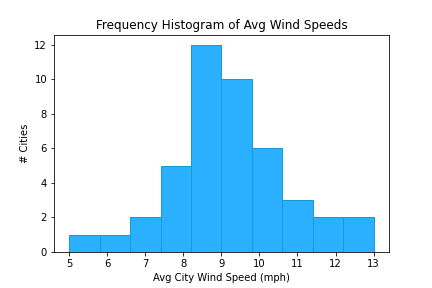
\includegraphics[width=0.5\textwidth]{1_2_a.png}
        \end{figure}
        
        \item Yes, the high wind totals are consistent with the fact that Mt. Washington, New Hampshire is on a mountain.
        
        \item 24.44\% of cities are windier than Chicago.
        
        \item No, since 24.44\% of other cities in our sample are windier than Chicago. Therefore Chicago is not unusually windy when you consider how unusually windy other supposed outliers are such as Mt. Washington, NH. Chicago is windier than most cities, but is not unusually windy compared to cities in our sample.
        
    \end{enumerate}
        
\subsection*{Problem 1.3}
    \begin{figure}[H]
    \centering
    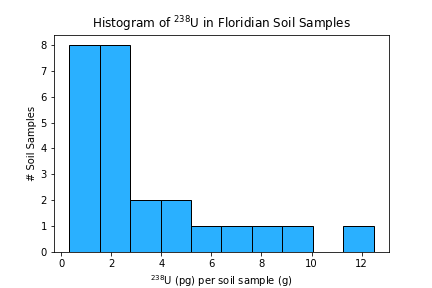
\includegraphics[width=0.5\textwidth]{1_3.png}
    \end{figure}
        
\subsection*{Problem 1.4}
    \begin{enumerate}[label=(\alph*).]
        \item 
        \begin{figure}[H]
        \centering
        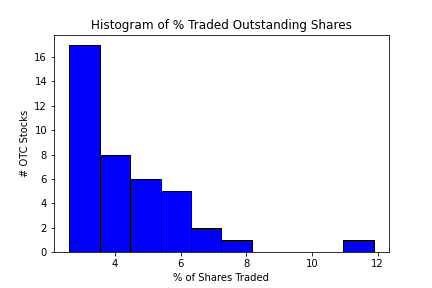
\includegraphics[width=0.5\textwidth]{1_4_a.png}
        \end{figure}
        
        \item 0.4500 of top 40 stocks traded more than 4\% of outstanding shares.
        
        \item The likelihood that a randomly selected stock from our sample traded more than 5\% of outstanding shares is 0.7250.
        
        
    \end{enumerate}

\subsection*{Problem 1.5}
    \begin{enumerate}[label=(\alph*).]
        \item The categories with the largest proportion of students is (-2.45, 2.65) and (2.65, 2.85). 
        
        \item In each category, there are 7/30 of total sampled students.
        
        \item 3 + 3 + 3 + 7 = 16. \\
        
        16/30 students had a GPA less than 2.65. \\
        
        
    \end{enumerate}

\subsection*{Problem 1.6}
    \begin{enumerate}[label=(\alph*).]
        \item The model category is the '2 quarts of milk' category.
        
        \item 9/25, or 0.36 of the 25 families purchased more than 2 quarts of milk.
        
        \item 23/25, or 0.92 of the 25 families purchased more than 0 and fewer than 5 quarts of milk.

\subsection*{Problem 1.7}
    \begin{enumerate}[label=(\alph*).]
        \item A curve with two peaks; the graph is bimodal.
        
        \item The two peaks are unusual compared to previous data we've analyzed.
        
        \item The intervals are too small, failing to capture the trend of the data. \\
        
        Notice how the two peaks of the histogram are close to each other on the x-axis. This suggests that the two peaks should actually be represented by one peak. To fix this issue, we should increase the size of the categories.
    \end{enumerate}
    
\subsection*{Problem 1.8}
    \begin{enumerate}[label=(\alph*).]
        \item
        \begin{figure}[H]
        \centering
        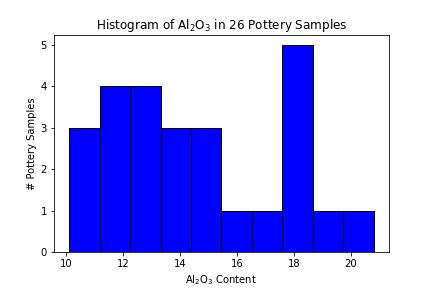
\includegraphics[width=0.5\textwidth]{1_8_a.png}
        \end{figure}
        
        \item The histogram is bimodal, but unlike in Problem 1.7, this does not appear to be an issue of category size. The data suggests that there are two common Al$_2$O$_3$ values, not one. This is likely due to how Island Thomas and Ashley Rails pottery have larger Al$_2$O$_3$ values than Llanederyn and Calcidot pottery.
        
    \end{enumerate}
        
        
    \end{enumerate}
\end{document}